\section{Gentle Path (Working Title)}

In this section the paths that were optimized in section \ref{subsec:long_paths} will be tracked. Both the ground path and the optimized path will be tracked, so that the optimized path can be compared to the original path. In Figure \ref{fig:sim_tracking} the UAV position is shown together with the optimized path that it were to track, and it shows that the simple LOS guidance written in DUNE has satisfactory performance. The LOS distance was set to $150$m by trial and failure.

\begin{figure}
	\makebox[\textwidth][c]{
	\subfloat[UAV position]{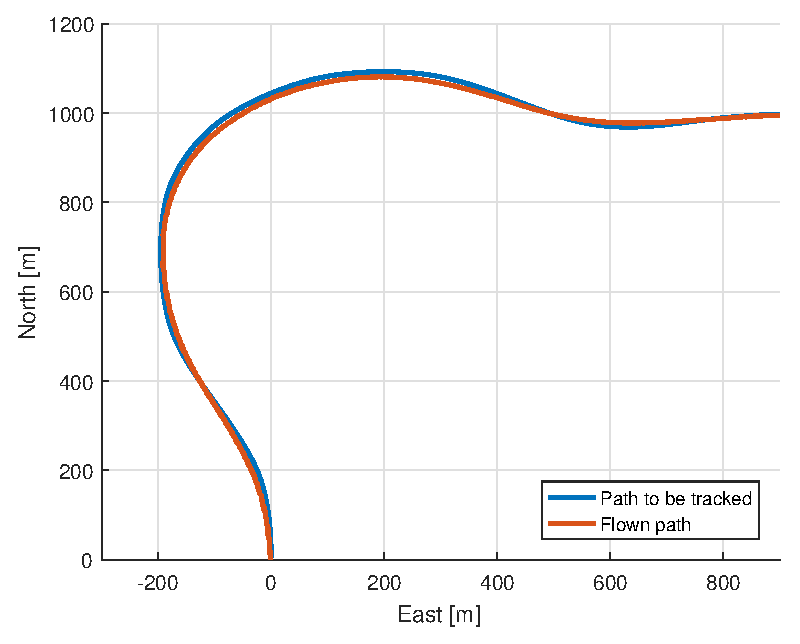
\includegraphics[width=0.5\textwidth, keepaspectratio=true]{../../results/sim/easy_path/fig_lin/tracking.eps}}
	\qquad
	\subfloat[Camera position]{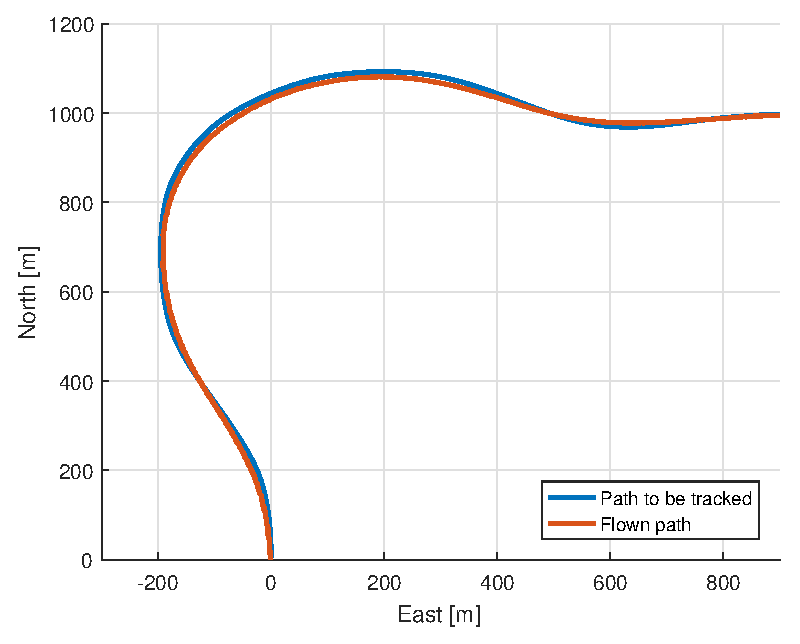
\includegraphics[width=0.5\textwidth, keepaspectratio=true]{../../results/sim/easy_path/fig_lin/tracking.eps}}}
	\caption{Result when tracking the optimized path.}
	\label{fig:sim_tracking}
\end{figure}


\subsection{Linear Path}

The result of tracking the linear ground path and the optimized path can be seen in Figure \ref{fig:lin_sim_res}. It is clear that when tracking the ground path the biggest problem is that the path that is being tracked is linear, giving the aircraft abrupt changes in the roll angle. When tracking the optimized path on the other hand, the are no abrupt changes in the roll angle. The smooth referance path gives a smooth flight path, and the camera centre point stays focused on the ground path without any major deviations.

\begin{figure}
	\makebox[\textwidth][c]{
	\subfloat[Tracking the ground path]{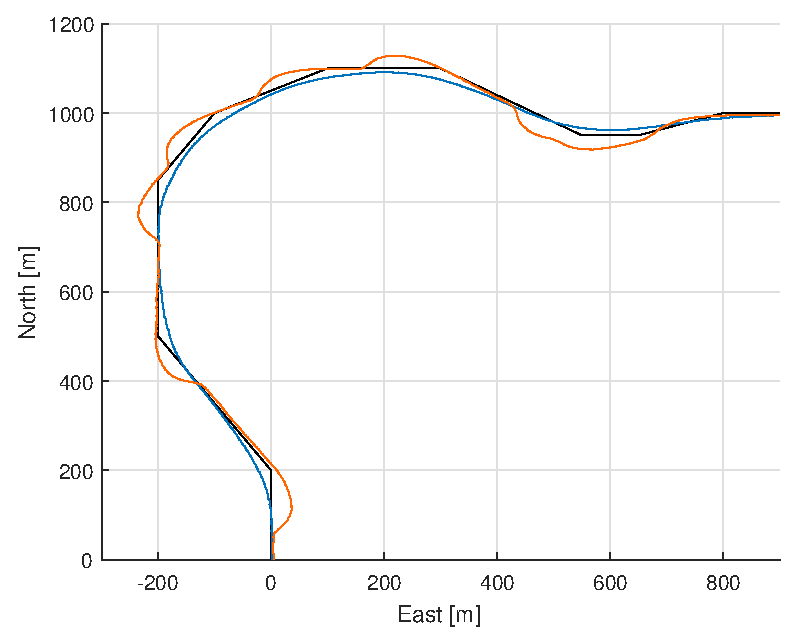
\includegraphics[width=0.8\textwidth, keepaspectratio=true]{../../results/sim/easy_path/fig_lin/path_run.eps}}}
	\makebox[\textwidth][c]{
	\subfloat[Tracking the optimized path]{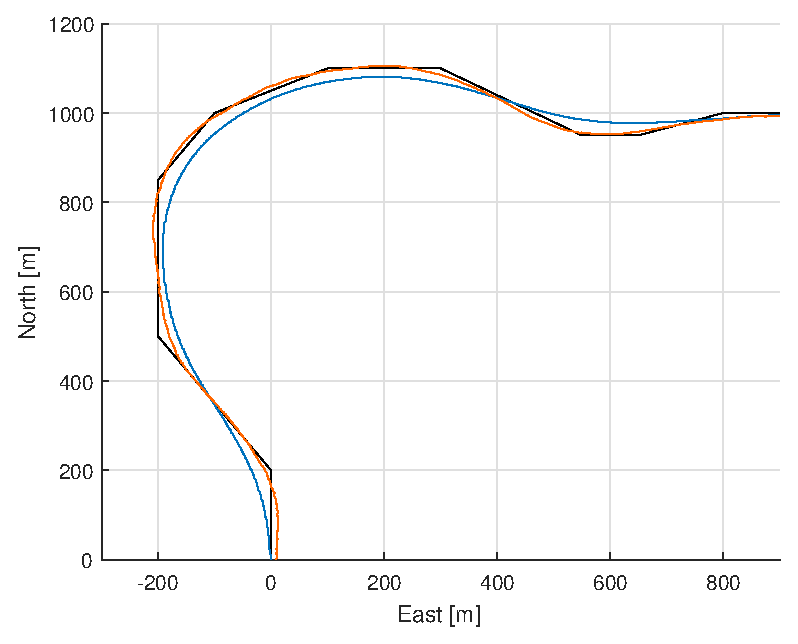
\includegraphics[width=0.8\textwidth, keepaspectratio=true]{../../results/sim/easy_path/fig_lin/pos_run.eps}}}
	\caption{The result when tracking the ground path and the optimized path.}
	\label{fig:lin_sim_res}
\end{figure}


\subsection{Curved Path}

The results for tracking the curved path is very similar to the results for the linear tracking. The tracking of the ground path is less abrupt, but the optimized path has a much smoother path in this case as well. 

\begin{figure}
	\makebox[\textwidth][c]{
	\subfloat[Tracking the ground path]{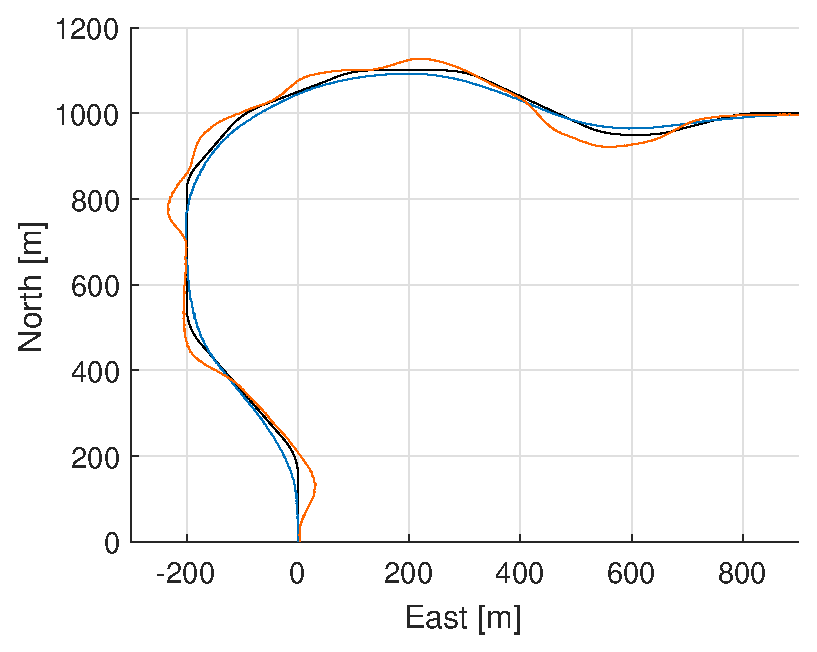
\includegraphics[width=0.8\textwidth, keepaspectratio=true]{../../results/sim/easy_path/fig_cur/path_run.eps}}}
	\makebox[\textwidth][c]{
	\subfloat[Tracking the optimized path]{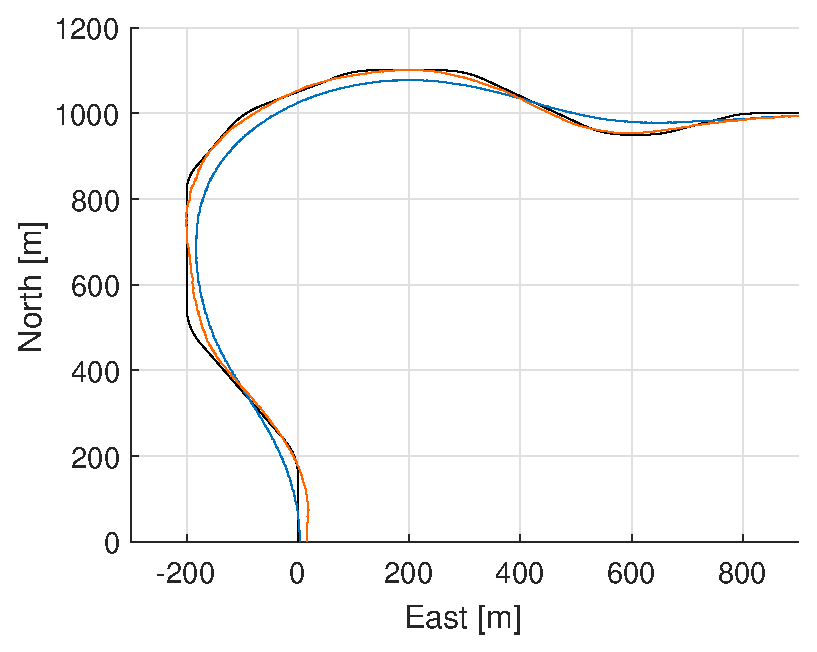
\includegraphics[width=0.8\textwidth, keepaspectratio=true]{../../results/sim/easy_path/fig_cur/pos_run.eps}}}
	\caption{The result when tracking the ground path and the optimized path.}
	\label{fig:cur_sim_res}
\end{figure}


\subsection{Linear VS. Curved}

\begin{table}
\centering
\begin{tabular}{l r r r}
    \hline
    & Mean & Max  & STD \\
    \hline
    Optimized Curved Path & 4.0366m & 21.6539m & 5.0647m \\
    Optimized Linear Path & 3.5139m & 18.4791m & 4.0691m \\
    Ground Curved Path & 8.0423m & 36.4857m & 10.4101m \\
    Ground Linear Path & 7.9658m & 40.5172m & 11.2268m \\
    \hline
\end{tabular}
\caption{Mean error, max error and the standard deviation between camera centre point and ground path when tracking the path.}
\label{tab:sim_easy}
\end{table}

The statistics for the simulations of the paths can be seen in Table \ref{tab:sim_easy}, and they show that the performance when tracking the linear path is better than when trackin the curved path. The mean deviance is $0.5$m shorter for the linear path than for the curved path, and the maximum deviance when tracking the linear path is a little more than $3$m better. This is opposite of the results when optimizing the paths, where the curved path had a better tracking. It is also worth noting that mean error when optimizing the paths was bigger than the mean error when simulating the paths, and tracking the optimized paths give a considerably better result than tracking the ground path.